\documentclass[a4paper,12pt]{article}
%%%%%%%%%%%%%%%%%%%%%%%%%%%%%%%%%%%%%%%%%%%%%%%%%%%%%%%%%%%%%%%%%%%%%%%%%%%%%%%%%%%%%%%%%%%%%%%%%%%%%%%%%%%%%%%%%%%%%%%%%%%%%%%%%%%%%%%%%%%%%%%%%%%%%%%%%%%%%%%%%%%%%%%%%%%%%%%%%%%%%%%%%%%%%%%%%%%%%%%%%%%%%%%%%%%%%%%%%%%%%%%%%%%%%%%%%%%%%%%%%%%%%%%%%%%%
\usepackage{eurosym}
\usepackage{vmargin}
\usepackage{amsmath}
\usepackage{graphics}
\usepackage{epsfig}
\usepackage{subfigure}
\usepackage{fancyhdr}
\usepackage{listings}
\usepackage{framed}
\usepackage{graphicx}
\usepackage{amsmath}
\usepackage{chngpage}
%\usepackage{bigints}

\setcounter{MaxMatrixCols}{10}

\begin{document}
\large
%nbviewer
%FAQ
%IPython
%Jupyter
%bokeh-notebooks   tutorial
 	
\section{Bokeh Tutorial — bokeh.plotting interface}
This section of the tutorial covers the bokeh.plotting interface. This interface is a "mid-level" interface, and the main idea can be described by the statement:

Starting from simple default figures (with default tools, grids and axes), add markers and other shapes whose visual attributes are tied to data.
We will see that it is possible to customize and change all of the defaults, but having them means that it is possible to get up and running very quickly.

\subsection{Imports and Setup}
When using the \texttt{bokeh.plotting} interface, there are a few common imports:
\begin{itemize}


\item Use the figure function to create new plot objects to work with.
\item Call the functions \texttt{output\_file}, \texttt{output\_notebook}, and \texttt{output\_server} (possibly in combination) to tell Bokeh how to display or save output.
\item Execute show and save to display or save plots and layouts.
\end{itemize}


\begin{framed}
\begin{verbatim}
In [1]:
from bokeh.io import output_notebook, show
from bokeh.plotting import figure
\end{verbatim}
\end{framed}
In this case, we are in the Jupyter notebook, so call \texttt{output\_notebook()}. We only need to call this once, and all subsequent calls to \texttt{show()} will display inline in the notebook.
\begin{framed}
	\begin{verbatim}
In [2]:
output_notebook()
BokehJS successfully loaded.
\end{verbatim}
\end{framed}
\subsection{Some Basic Scatter Plots}
In this section you will see how to use Bokeh's various marker types to create simple scatter plots.
\begin{framed}
	\begin{verbatim}
In [3]:
# create a new plot with default tools, using figure
p = figure(plot_width=400, plot_height=400)

# add a circle renderer with a size, color, and alpha
p.circle([1, 2, 3, 4, 5], [6, 7, 2, 4, 5], size=15, line_color="navy", fill_color="orange", fill_alpha=0.5)

show(p) # show the results
\end{verbatim}
\end{framed}
All Bokeh markers accept size (measured in screen space units) as a property. Circles also have radius (measured in "data" space units).

\begin{framed}
\begin{verbatim}
In [4]:
# EXERCISE: Try changing the example above to set a `radius` value instead of `size`
To scatter square markers instead of circles, you can use the square method on figures.

In [5]:
# create a new plot using figure
p = figure(plot_width=400, plot_height=400)

# add a square renderer with a size, color, alpha, and sizes
p.square([1, 2, 3, 4, 5], [6, 7, 2, 4, 5], size=[10, 15, 20, 25, 30], color="firebrick", alpha=0.6)

show(p) # show the results
\end{verbatim}
\end{framed}
Note that in the example above, we are also specifying different sizes for each individual marker. In general, all of a glyph's properties can be "vectorized" in this fashion. Also note that we have passed color as a shorthand to set both the line and fill colors easily at the same time. This is a convenience specific to \texttt{bokeh.plotting}.

% </table>
%================================================================ %
There are many marker types available in Bokeh, you can see details and example plots for all of them in the reference guide by clicking on entries in the list below:
\begin{framed}
\begin{verbatim}
asterisk()
circle()
circle_cross()
circle_x()
cross()
diamond()
diamond_cross()
inverted_triangle()
square()
square_cross()
square_x()
triangle()
x()
\end{verbatim}
\end{framed}
\begin{framed}
	\begin{verbatim}
In [6]:
# EXERCISE: Plot some different markers in this cell
Basic Line Plots
In [7]:
# create a new plot (with a title) using figure
p = figure(plot_width=400, plot_height=400, title="My Line Plot")

# add a line renderer
p.line([1, 2, 3, 4, 5], [6, 7, 2, 4, 5], line_width=2)

show(p) # show the results
\end{verbatim}
\end{framed}
\begin{figure}[h!]
\centering
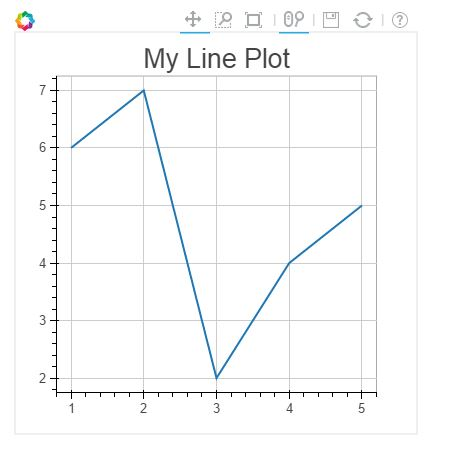
\includegraphics[width=0.7\linewidth]{images/01-BasicPlot-LinePlot}
\caption{}
\label{fig:01-BasicPlot-LinePlot}
\end{figure}

The example below shows how to use the \texttt{image\_rgba} method to display raw RGBA data.

Note: This example makes use of the NumPy library
\begin{framed}
	\begin{verbatim}
In [8]:
from __future__ import division
import numpy as np

# set up some data
N = 20
img = np.empty((N,N), dtype=np.uint32)
view = img.view(dtype=np.uint8).reshape((N, N, 4))
for i in range(N):
    for j in range(N):
        view[i, j, 0] = int(i/N*255) # red
        view[i, j, 1] = 158          # green
        view[i, j, 2] = int(j/N*255) # blue
        view[i, j, 3] = 255          # alpha
        
# create a new plot (with a fixed range) using figure
p = figure(x_range=[0,10], y_range=[0,10])

# add an RGBA image renderer
p.image_rgba(image=[img], x=[0], y=[0], dw=[10], dh=[10])

show(p) # show the results
\end{verbatim}
\end{framed}
%======================================================================================== %
\newpage
\section{Other Kinds of Glyphs}
Bokeh supports many other kinds of glyphs. You can click on the User Guide links below to see how to create plots with these glyphs using the \texttt{bokeh.plotting} interface.

\begin{itemize}
\item Rectangles and Ovals
\item Segments and Rays
\item Wedges and Arcs
\item Specialized Curves
\end{itemize}

%	In [9]:
%  # EXERCISE: Plot some of the other glyph types, following the examples in the User Guide. 
\subsection{Plots with Multiple Glyphs}
It is possible to combine more than one glyph on a single figure. You just need to call multiple glyph methods on one figure object:
\begin{framed}
	\begin{verbatim}
In [10]:
# set up some data
x = [1, 2, 3, 4, 5]
y = [6, 7, 8, 7, 3]

# create a new plot with figure
p = figure(plot_width=400, plot_height=400)

# add both a line and circles on the same plot
p.line(x, y, line_width=2)
p.circle(x, y, fill_color="white", size=8)

show(p) # show the results

\end{verbatim}
\end{framed}
\begin{figure}[h!]
\centering
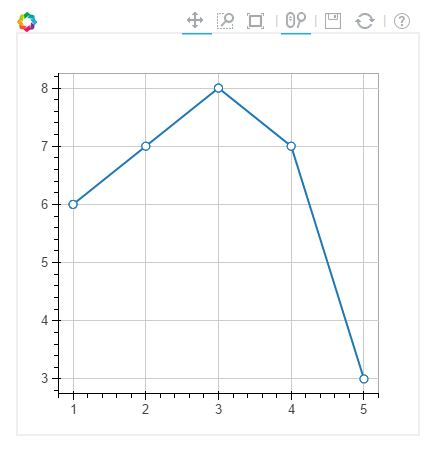
\includegraphics[width=0.7\linewidth]{images/01-BasicPlot-LinePlot-2}
\caption{}
\label{fig:01-BasicPlot-LinePlot-2}
\end{figure}

\end{document} 
%Back to top
%This web site does not host notebooks, it only renders notebooks available on other websites.
%
%Delivered by Fastly, Rendered by Rackspace
%
%nbviewer GitHub repository.
%
%nbviewer version: 03d6df0
%
%IPython version: 4.0.0
%
%Rendered in a few seconds
